\documentclass[]{article}
\usepackage{graphicx}
\graphicspath{ {./images/} }
\usepackage{amsthm}
\newtheorem{mydef}{Definition}[section]
\usepackage{amsfonts}
\usepackage{amsmath}
\usepackage[ruled,linesnumbered]{algorithm2e}

%opening
\title{Master Thesis --  Math Formalization}
\author{Kefang Ding} 
\date{9 Nov 2018}

\begin{document}

\maketitle

\hrulefill
\hrulefill 

\begin{abstract}
This article defines the mathematical formalization of algorithm, which is used to add long-term dependency in model repair by incorporating negative information. The following sections are organized in this way. Section 1 introduces the problems to solve. Section 2 gives formal definitions. Section 3 describes the algorithm to use. 
\end{abstract}

\section{Introduction}
The inputs for process model repair include one existing process model, an corresponding event log and a set of KPIs for the data evaluation in event log. After applying Directly-Following-Graph-based,abv, dfg-method, repair algorithm, a model with high fitness is generated. However, dfg-method can't discover, change the long-term dependency in the model, which makes the model less precise. \\
With concept Long-term dependency, it describes the dependency between activities, where the execution of one activity affects the execution of another activities later. This dependency  relates the choices structure in model, xor, loop and or structure. due to the complexity of or structure, this article only focus on the long-term dependency in xor and loop structures and introduces an algorithm to deal with this problem. \\
The inputs for this algorithm are,
\begin{itemize}
	\item Repaired model in process tree
	\item Event log with positive and negative labels
\end{itemize}
The output of this algorithm is: 
\begin{itemize}
	\item Repaired model in petri net with long-term dependency
\end{itemize}

\section{Definitions}
In this section, the related definitions are listed. Process Tree is one input for this method. To specify the process tree, the definitions involved in tree are reviewed at first.
\begin{mydef}[Tree]
	Let $ \mathbb{N} $ be a finite set of entities, a tree is a collection of entities called nodes, which are connected by edges. A tree T is,
	\[
	\begin{array}{ rll}
		\circ&t(\emptyset) & \mbox{with } t\; has\; no\; outgoing\; edge;\\
		\circ&t(T_1,T_2,...,T_n) & \mbox{with } i,n\in \mathbb{N}, i \leq n ,T_i\;is\; a\; tree.
	\end{array}
	\]
\end{mydef}
For convenience, we call $T_i$ is a child of $t(T_1,T_2,...,T_n)$, marked as $P(t,T_i)$, $t(T_1,T_2,...,T_n)$ is one parent of $T_i$. The root of tree is defined as one node, without any parent. A pat
For any node in a tree, its ancestor and descendant is defined as:
\begin{mydef}[Ancestor]
	An ancestor for a node t is a node A in a tree, if 
	\[ A\; is\; the\; parent\; of\; t \] or
	\[ \exists t_1,t_2..t_n,n\in \mathbb{N}, i < n, P(A,t_1)\land P(t_i,t_{i+1}) \land P(t_n,t) \]
\end{mydef}
A descendant for a node t is a node D, if t is the ancestor of D. For two nodes t and s, if t is the ancestor of s, we have A(t,s) true. The similar situation for descendant.
\begin{mydef}[Least Common Ancestor]
	A least common ancestor for node $s$ and node $t$ in a tree is a node n, where 
	\[A(n,s) \land A(n,t) \land \exists! m A(n,m) \land A(m,s) \land A(m,t) \]
\end{mydef}
Process tree is a specification of tree in context of process mining. It describes the block-structured process model. 
\begin{mydef}[Process Tree]
	Let $ A \subseteq \mathbb{A} $ be a finite set of activities with $\tau \in \mathbb{A}$, $\bigoplus \subseteq \{\rightarrow, \times, \land, \cup \footnote{it means the loop operator due to difficulty to print out the real loop symbol}\}$ be the set of process tree operators. 
	\begin{itemize}
		\item $Q=a$ is a process tree with $a\in A$, and 
		\item $Q= \oplus (Q_1 , Q_2 ,.. Q_n)$ is a process tree with $\oplus \in \bigoplus$, $Q_i$ is a process tree, $i\in{1,2,..,n}, n\in \mathbb{N}$. 
	\end{itemize}
\end{mydef}
Process tree operators represents different block relation of each subtree. Their semantics are listed below. 
\begin{mydef}[Operator Semantics] 
	The semantics of operators $\bigoplus \subseteq {\rightarrow, \times, \land, \cup}$ are,
	\begin{itemize}
		\item if $Q= \rightarrow(Q_1 , Q_2 ,.. Q_n)$, the subtrees have sequential relation and are executed in order of $Q_1,Q_2,..Q_n$
		\item if $Q= \times(Q_1 , Q_2 ,.. Q_n)$,  the subtrees have exclusive relation and $Q_1,Q_2,..Q_n$  only one subtree of them can be executed.
		\item if $Q= \land (Q_1 , Q_2 ,.. Q_n)$,  the subtrees have parallel relation and $Q_1,Q_2,..Q_n$ they can be executed in parallel.
		\item if $Q= \cup(Q_1 , Q_2 ,.. Q_n)$,  the subtrees have loop relation and $Q_1,Q_2,..Q_n with n\geq2$,$Q_1$ is the do-part and is executed at least once, $Q_2,..Q_n$ are redo part and have exclusive relation.
	\end{itemize}
\end{mydef}
In the following figure\ref{fig:not_nested_overview}, it's a typical process tree. It describes a business model, which includes the sequential, exclusive and parallel relations among the activities.  The model is sound. 
%-- add one process tree graph here. 
\begin{figure}[h!]
	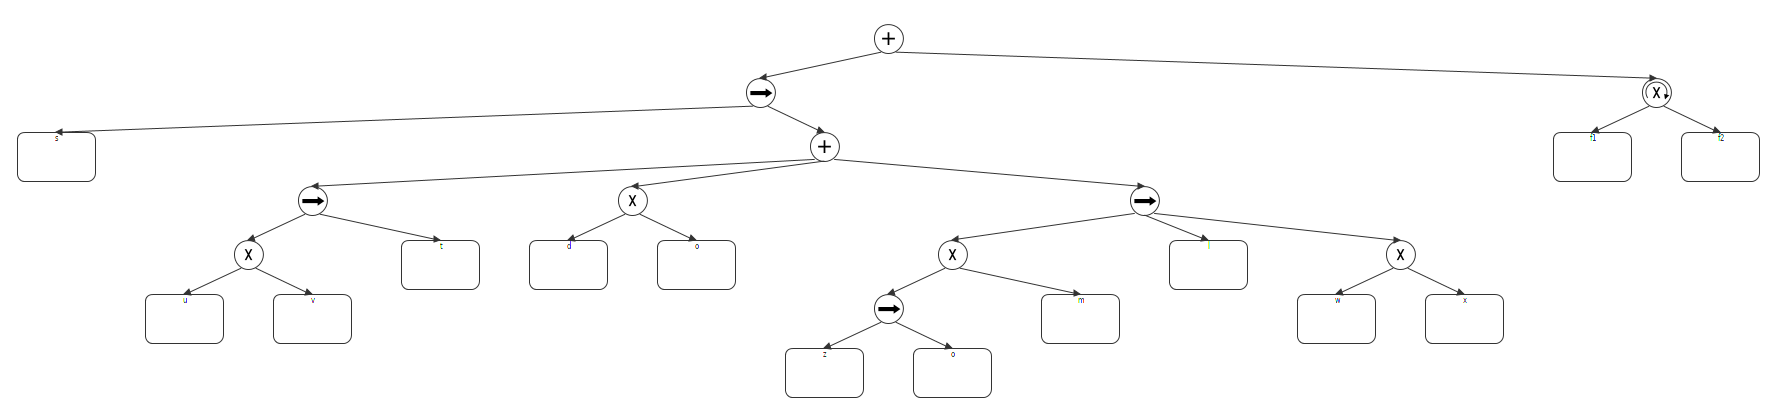
\includegraphics[width=\textwidth]{PT01_Not_Nested_Overview.png}
	\caption{Process Tree With All Operators}
	\label{fig:not_nested_overview}
\end{figure}
%-- but we just use the process tree to build the model, actually not to add the long-term dependency on it
During model execution, we observe that, in some situations, the execution of events in the exclusive block has influence on the execution of events later, which is called long-term dependency. In the following, the focus is to deal with long-term dependency in the model. 
For the sake of convenience, exclusive block is abbreviated as xor block; also, the subtree of xor block is defined as xor branch. 
\begin{mydef}[xor branch]
   $Q= \times(Q_1 , Q_2 ,.. Q_n)$, $Q_i$ is one xor branch with respect to Q. For convenience, we use X to represent one xor branch, and record it $X\in XOR_{Q}$
\end{mydef}
Due to the different structure of xor branch, we drive two properties of xor block, purity and nestedness.
\begin{mydef}[XOR Purity]
	A xor block is pure if and only $\forall X\in XOR_Q, Leaf(X) \rightarrow True$. Else, the block is unpure.
\end{mydef}
\begin{mydef}[XOR Nestedness]
	A xor block is nested if and only $\exists X XOR(X) \land Ct(XOR_Q,X) $, where $Ancestor(XOR_Q,X)$ represents $XOR_Q$ is an ancestor of X in the process tree.
\end{mydef}
In the Figure\ref{fig:xor_branch_variants}, xor block Xor:(c1,c2) are pure and not nested, since all the xor branches are leaf node, but xor block Xor:(a,Seq:(b,Xor:(c1,c2))) is impure and nested with Xor:(c1,c2). 
\begin{figure}[h!]
	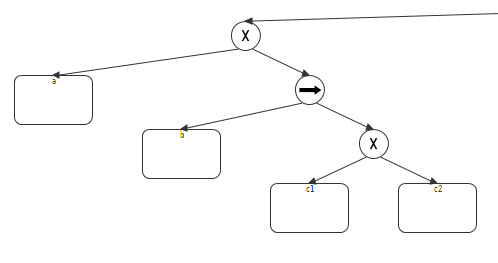
\includegraphics[width=\textwidth]{PT02_xor_nested_and_pure.png}
	\caption{XOR branch variants}
	\label{fig:xor_branch_variants}
\end{figure}

Due to the definition, the least common ancestor of X:(c1,c2) and b in Figure \ref{fig:xor_branch_variants} is Seq:(b,Xor:(c1,c2)).\\
Long-term dependency is associated with choices in xor block, namely each xor branch in xor block. To define it, the following concepts are in need. The first is the order of xor block in sequential structure.
\begin{mydef}[Order of xor block]
	$xor_A$ is before $xor_B$, written in $xor_A \prec xor_B$, if and only if one ancestor branch of $xor_A$ is before the ancestor of $xor_B$ in sequential block. 
\end{mydef}
We can drive the order of xor block in Figure\ref{fig:not_nested_overview}. $Xor:(Seq:(z,o),m) \prec Xor:(w,x)$ , because the least common ancestor of them is sequential, so they are always executed in an order. However, for Xor:(u,v) and Xor:(d,o), their least common ancestor is parallel, so they don't have any execution order. If they are in loop as in Figure\ref{fig:xor_in_loop}, we define the xor in do part is before the xor in redo part, namely $Xor:(f3,f4) \prec Xor:(f6,f7)$.
\begin{figure}[h!]
	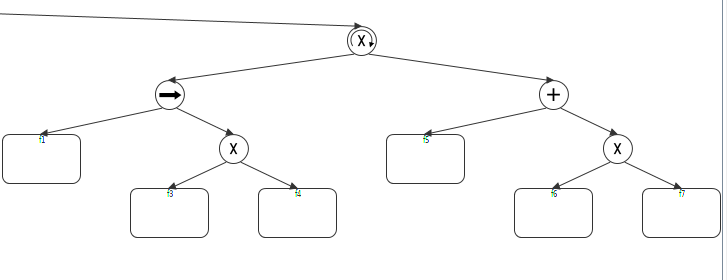
\includegraphics[width=\textwidth]{PT03_xor_in_loop.png}
	\caption{XOR in loop}
	\label{fig:xor_in_loop}
\end{figure}
With the order definition, we introduce the definition for xor pair.
\begin{mydef}[XOR Pair]
	$xor_A$ and $xor_B$ is an xor pair, written in XOR\_Pair($XOR_A, XOR_B$), if $XOR_A \prec XOR_B$.
\end{mydef}
\begin{mydef}[Event Frequency]
	Event Frequency in an event log l is an atom $F_{l}(a,freq)$ where a is an event,$a \in A$  and freq is the happened frequency in integer for event a.
\end{mydef}
In the recursive definition from the above, we can define the xor branch frequency in an event log.
\begin{mydef}[Xor Branch Frequency]
	Xor branch frequency in event log l is $F_{l}(X,freq)$ where X is an xor branch, and freq is the happened frequency in integer for xor branch X.
\end{mydef}
\begin{mydef}[Supported Connection of Xor branches\footnotemark]
Given an event log, xor branch X and Y have supported connection over a threshold t, $SC_{l}(X,Y,t)$ if and only if \[ for \space X \in xor_S, Y \in xor_T, \exists freq, F_{l}(X,freq) \land F_{l}(Y,freq) \land freq \geq t. \]
\end{mydef}
\footnotetext{here we don't point out the negative instances use. With negative information, it is: $freq(pos) \geq t^{1} \land freq(pos) - freq(neg)\geq t^{2} $}
After introduction of supported connection of xor branches, we can define the long-term dependency. 
\begin{mydef}[Long-term Dependency in XOR block]
	$xor_S$ and $xor_T$ have long-term dependency over an threshold t w.r.t. an event log, $LT(xor_S, xor_T,t) $ if and only if 
	\begin{itemize}
		\item there are at least two xor blocks in model, $xor_S \neq xor_T \land xor_S \prec xor_B$
		\item $\exists X \in XOR_S, \exists Y \in XOR_T, \lnot SC_{l}(X,Y,t)$. 
	\end{itemize}
\end{mydef}
In this context, we define the long-term dependency between xor branches.
\begin{mydef}[Long-term Dependency in XOR branches]
	Xor branch X and Y have long-term dependency over an threshold t w.r.t. an event log, $LT(X,Y,t) $ if and only if  
	\[\exists X \in XOR_S, \exists Y \in XOR_T, LT(XOR_S, XOR_T, t) \land SC(X,Y,t) \rightarrow LT(X,Y,t).\]	
\end{mydef}

\section{Algorithm}
According to the long-term dependency definition, we propose our algorithm to discover long-term dependency. Because the purity, nestedness and its position in process tree, we need to deal with long-term dependency in different situations.However, due to the complexity, the algorithm focuses only on the binary long-term dependency of xor block, which means, we only create xor pair of $XOR_X and XOR_Y$, marked with where 
\[ \exists ! XOR_Z, \: XOR_S \prec XOR_T \rightarrow XOR_S \prec XOR_Z \land XOR_Z \prec XOR_Y \]
The general steps of algorithm is in the following. 

\begin{algorithm}[H]
	\SetAlgoLined
	\KwResult{Discover Long-term Dependency In Model}
	create a list including all xor pairs in process tree\;
	\While{pair in xor pair list}{
		\If{this pair has no LT dependency}{
			remove this pair from xor pair list\;
		}
	}
	transfer process tree into Petri net\;
	add places in Petri net for every branch pair with long-term dependency\;
	\caption{General steps to add long-term dependency}
\end{algorithm}
We give more details about the each steps in the next parts.
\subsection{Create All XOR Pairs}
Given one process tree with xor blocks, we create XOR pairs in such situations. 
\subsubsection{Sequential XOR Block Without Nested XOR Block}
In this situation, we only consider the model without nested xor block and create xor pair only in sequential order, like in the figure.
%% insert one graph to explain this situation and then create those pairs. 
To get the long-term dependency, the begin and end node in one branch is of importance, it marks the execution of this xor branch. In implementation, we have the following variants of branch. 
\begin{itemize}
	\item xor branch is a leaf node a, beginNode = endNode = a;
	\item xor branch is sequential, marked as Seq, beginNode = firstChild(Seq), endNode = lastChild(Seq);
	\item xor branch is parallel, marked as Parallel, to reduce complexity, we add one sequential node for structure modification; silent activities to the begin and end of sequential structure, and parallel kept in the middle. The xor branch goes back to sequential handle.
	\item xor branch is loop, marked as loop, the similar solution like in parallel, one sequential node is created to keep the loop structure in the middle, two silent activities are divided into the begin and end parts.
\end{itemize}
We visit the process tree in depth-first, and create xor pair for two xor blocks $XOR_S$ and $XOR_T$, if they are in order.
\subsubsection{ Sequential XOR Block With Nested XOR Block}
For the model with nested xor block like Xor:(a,Seq:(b,Xor:(c1,c2))) in Figure\ref{fig:xor_branch_variants} , the nested block needs a redefinition for its branch. 
\begin{itemize}
	\item If one of its xor branches contains no xor block, this branch is kept;
	\item if one xor branch has xor block, called sub xor block, all branches without xor block in the sub xor block should be added to the nested block.  
\end{itemize}
This procedure is called nested xor block folding. After we fold all xor block, we create xor pair.  	
\subsubsection{Parallel XOR Block}
Given a model with xor blocks in parallel relation and event log which supports long-term dependency, we need to add long-term dependency on the model. There are some situations.
\begin{itemize}
	\item in each parallel branch, there exists one xor block, long-term pattern is one xor branch decides the choices of another xor
\end{itemize}
%% put some figures to explain it in process tree
%% some situations for this problem by using petri net
  %% in three xor in parallel and then one in sequence, but then how to do it ?? We also need to anaglyze it   
\subsubsection{Loop XOR Block}
Long-term dependency divers in loop block as listed below. 
\begin{itemize}
	\item xor before loop block, several choices for redo part in loop block, as shown in Figure;; With different support, we can have different long-term dependency.
	\item xor before loop block, xor in do part of loop block
	\item xor before loop block, xor in redo part of loop block
	\item xor in loop block do and redo part
	\item xor before loop, xor in do part and redo part
\end{itemize}
We only deal with those situations with like this %put it in one graph and write down the pattern%
\begin{align}
<A, L_{1}^{*} || L_{2}^{*} || E> \\
<B, L_{1}^{*} || L_{2}^{*} || E>
\end{align}
\subsection{Check if the pair has LT Dependency}
After getting all the xor pairs from the model, we check if the pair has long-term dependency with corresponding event log.


\subsection{Transfer Process Tree into Petri Net}
By using already existing application, the process tree is transferred into Petri net without long-term dependency connection. The silent nodes from the last step are also shown in the Petri net as silent transitions.
However, if we discover the long-term dependency directly on the Petri net, we don't need the process tree transformation. In this article, the steps are quite detailed;; But the definitions are general enough for design. 
\subsection{Add Long-term dependency}
In Petri net, long-term dependency is addressed by adding extra places and silent transitions in xor pair.  
% one figure is in need to describe this% 
\begin{algorithm}
	\SetAlgoLined
	Add places after xor join structure \;
		\ForEach{xor branch in xor pair}{
			add one place after its branch end node}    
	Add places before xor split structure\;
	Add silent transition to connect places\;
	\caption{Add long-term dependency in xor pair}
\end{algorithm}
\subsubsection{Sequential}

\subsubsection{Parallel}

\subsubsection{Loop}

\end{document}
